% Ukázky specializovaných NLP úloh (starší screenshoty), dříve součást nlp.tex

% ----------------------------------------------------------------------------

\begin{frame}{Vyhledávání odpovědí na otázky}

    \centering
    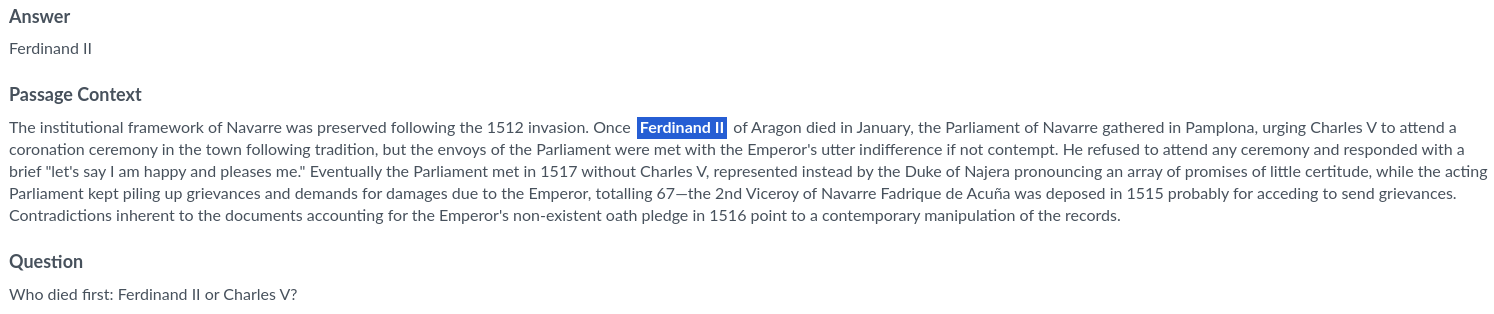
\includegraphics[scale=.26]{img/qa.png} \\
    {\tiny Screenshot z~dema Allen Institute for AI \url{https://demo.allennlp.org/reading-comprehension/transformer-qa}}

\end{frame}

% ----------------------------------------------------------------------------

\begin{frame}{Kontrola pravopisu}

    \centering
    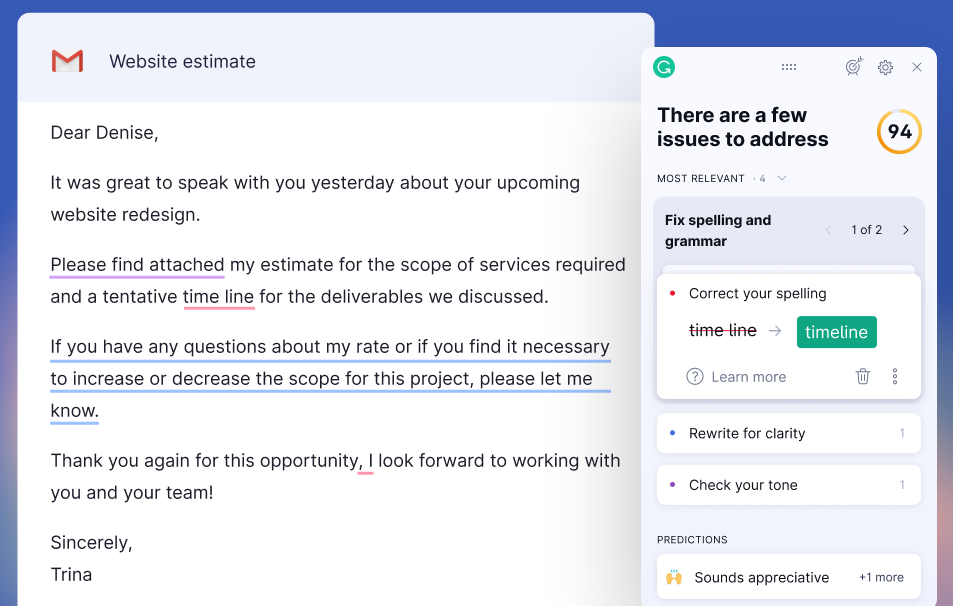
\includegraphics[scale=.3]{img/grammarly.png} \\
    {\tiny Zdroj: Webová reklama grammarly.com}

\end{frame}

% ----------------------------------------------------------------------------

\begin{frame}{Entity extraction}

    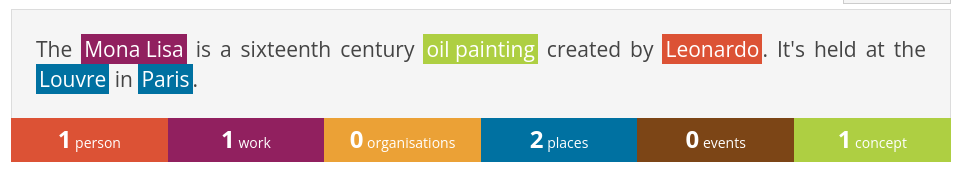
\includegraphics[scale=.4]{./img/mona_lisa.png} \\
    {\tiny Zdroj: \url{https://dandelion.eu/semantic-text/entity-extraction-demo}}

    \vspace{10pt}

    \visible<2->{Podúlohy:}
    \begin{enumerate}

        \item<3-> Named entity recognition: nalézt v~textu řetězce, co obsahují
            pojmenované entity

        \item<4-> Entity linking: co entity znamenají (první pád, odkaz do
            databáze/na Wikipedii)

    \end{enumerate}

\end{frame}

